\section{Resultados calculados}
La campaña ejecutó 2808 condiciones y 8424 ajustes. Hubo 0 ajustes fallidos y 6 condiciones sin convergencia completa. Cumplieron convergencia declarada y umbrales físicos 430 condiciones.
{\scriptsize\setlength{\tabcolsep}{3pt}
\begin{longtable}{p{.17\textwidth}p{.16\textwidth}p{.30\textwidth}rrr}
\caption{Menor error mediano de velocidad entre estimadores convergidos en todas las semillas declaradas. AP: semillas aceptadas físicamente.}\\
\toprule Caso & Ruido & Método & $e_u$ [\%] & $e_\omega$ [\%] & AP \\\midrule\endfirsthead
\toprule Caso & Ruido & Método & $e_u$ [\%] & $e_\omega$ [\%] & AP \\\midrule\endhead
taylor\_\allowbreak green & gaussiano & tls\_\allowbreak dmd\_\allowbreak helmholtz\_\allowbreak dealias & 1.684 & 7.143 & 3/3 \\
taylor\_\allowbreak green & impulsivo & rpca & $<0.001$ & 0.001 & 3/3 \\
taylor\_\allowbreak green & mixed & tls\_\allowbreak dmd\_\allowbreak helmholtz\_\allowbreak dealias & 1.697 & 7.463 & 3/3 \\
taylor\_\allowbreak green & spatial\_\allowbreak correlated & tls\_\allowbreak dmd\_\allowbreak helmholtz\_\allowbreak dealias & 3.126 & 5.036 & 3/3 \\
taylor\_\allowbreak green & temporal\_\allowbreak correlated & tls\_\allowbreak dmd\_\allowbreak helmholtz\_\allowbreak dealias & 6.877 & 29.209 & 0/3 \\
taylor\_\allowbreak green & column\_\allowbreak outliers & tls\_\allowbreak dmd\_\allowbreak helmholtz\_\allowbreak dealias & 1.782 & 7.417 & 3/3 \\
taylor\_\allowbreak green & student\_\allowbreak t & tls\_\allowbreak dmd\_\allowbreak helmholtz\_\allowbreak dealias & 1.706 & 7.633 & 3/3 \\
taylor\_\allowbreak green & heteroscedastic & tls\_\allowbreak dmd\_\allowbreak helmholtz\_\allowbreak dealias & 1.850 & 7.740 & 3/3 \\
taylor\_\allowbreak green & sensor\_\allowbreak drift & stable\_\allowbreak rpca & 19.429 & 4.125 & 0/3 \\
interacting\_\allowbreak vortices & gaussiano & tls\_\allowbreak dmd\_\allowbreak helmholtz\_\allowbreak dealias & 3.800 & 27.128 & 0/3 \\
interacting\_\allowbreak vortices & impulsivo & tls\_\allowbreak dmd\_\allowbreak helmholtz\_\allowbreak dealias & 3.901 & 27.574 & 0/3 \\
interacting\_\allowbreak vortices & mixed & tls\_\allowbreak dmd\_\allowbreak helmholtz\_\allowbreak dealias & 3.797 & 27.166 & 0/3 \\
interacting\_\allowbreak vortices & spatial\_\allowbreak correlated & tls\_\allowbreak dmd\_\allowbreak helmholtz\_\allowbreak dealias & 5.488 & 17.344 & 3/3 \\
interacting\_\allowbreak vortices & temporal\_\allowbreak correlated & tls\_\allowbreak dmd\_\allowbreak helmholtz\_\allowbreak dealias & 7.520 & 59.521 & 0/3 \\
interacting\_\allowbreak vortices & column\_\allowbreak outliers & rpca & 7.140 & 17.838 & 0/3 \\
interacting\_\allowbreak vortices & student\_\allowbreak t & tls\_\allowbreak dmd\_\allowbreak helmholtz\_\allowbreak dealias & 3.869 & 27.773 & 0/3 \\
interacting\_\allowbreak vortices & heteroscedastic & tls\_\allowbreak dmd\_\allowbreak helmholtz\_\allowbreak dealias & 3.834 & 27.568 & 0/3 \\
interacting\_\allowbreak vortices & sensor\_\allowbreak drift & identity\_\allowbreak helmholtz & 20.000 & $<0.001$ & 0/3 \\
decaying\_\allowbreak turbulence & gaussiano & tls\_\allowbreak dmd\_\allowbreak helmholtz\_\allowbreak dealias & 3.985 & 17.705 & 3/3 \\
decaying\_\allowbreak turbulence & impulsivo & rpca & 2.174 & 5.805 & 3/3 \\
decaying\_\allowbreak turbulence & mixed & tls\_\allowbreak dmd\_\allowbreak helmholtz\_\allowbreak dealias & 3.999 & 17.746 & 3/3 \\
decaying\_\allowbreak turbulence & spatial\_\allowbreak correlated & tls\_\allowbreak dmd\_\allowbreak helmholtz\_\allowbreak dealias & 5.754 & 10.801 & 3/3 \\
decaying\_\allowbreak turbulence & temporal\_\allowbreak correlated & tls\_\allowbreak dmd\_\allowbreak helmholtz\_\allowbreak dealias & 7.875 & 37.529 & 0/3 \\
decaying\_\allowbreak turbulence & column\_\allowbreak outliers & rpca & 5.056 & 8.473 & 3/3 \\
decaying\_\allowbreak turbulence & student\_\allowbreak t & tls\_\allowbreak dmd\_\allowbreak helmholtz\_\allowbreak dealias & 4.018 & 17.813 & 3/3 \\
decaying\_\allowbreak turbulence & heteroscedastic & tls\_\allowbreak dmd\_\allowbreak helmholtz\_\allowbreak dealias & 4.414 & 19.128 & 3/3 \\
decaying\_\allowbreak turbulence & sensor\_\allowbreak drift & rpca & 19.968 & 3.069 & 0/3 \\
oldroyd\_\allowbreak b\_\allowbreak 2d & gaussiano & tls\_\allowbreak dmd\_\allowbreak helmholtz\_\allowbreak dealias & 2.768 & 13.333 & 3/3 \\
oldroyd\_\allowbreak b\_\allowbreak 2d & impulsivo & rpca & 0.995 & 2.721 & 3/3 \\
oldroyd\_\allowbreak b\_\allowbreak 2d & mixed & tls\_\allowbreak dmd\_\allowbreak helmholtz\_\allowbreak dealias & 2.799 & 13.078 & 3/3 \\
oldroyd\_\allowbreak b\_\allowbreak 2d & spatial\_\allowbreak correlated & tls\_\allowbreak dmd\_\allowbreak helmholtz\_\allowbreak dealias & 4.203 & 8.810 & 3/3 \\
oldroyd\_\allowbreak b\_\allowbreak 2d & temporal\_\allowbreak correlated & tls\_\allowbreak dmd\_\allowbreak helmholtz\_\allowbreak dealias & 7.408 & 39.902 & 0/3 \\
oldroyd\_\allowbreak b\_\allowbreak 2d & column\_\allowbreak outliers & rpca & 4.010 & 6.436 & 3/3 \\
oldroyd\_\allowbreak b\_\allowbreak 2d & student\_\allowbreak t & tls\_\allowbreak dmd\_\allowbreak helmholtz\_\allowbreak dealias & 2.774 & 12.769 & 3/3 \\
oldroyd\_\allowbreak b\_\allowbreak 2d & heteroscedastic & tls\_\allowbreak dmd\_\allowbreak helmholtz\_\allowbreak dealias & 2.741 & 12.751 & 3/3 \\
oldroyd\_\allowbreak b\_\allowbreak 2d & sensor\_\allowbreak drift & stable\_\allowbreak rpca & 19.791 & 8.187 & 0/3 \\
fene\_\allowbreak p\_\allowbreak 2d & gaussiano & tls\_\allowbreak dmd\_\allowbreak helmholtz\_\allowbreak dealias & 2.770 & 13.337 & 3/3 \\
fene\_\allowbreak p\_\allowbreak 2d & impulsivo & rpca & 0.994 & 2.720 & 3/3 \\
fene\_\allowbreak p\_\allowbreak 2d & mixed & tls\_\allowbreak dmd\_\allowbreak helmholtz\_\allowbreak dealias & 2.801 & 13.082 & 3/3 \\
fene\_\allowbreak p\_\allowbreak 2d & spatial\_\allowbreak correlated & tls\_\allowbreak dmd\_\allowbreak helmholtz\_\allowbreak dealias & 4.204 & 8.815 & 3/3 \\
fene\_\allowbreak p\_\allowbreak 2d & temporal\_\allowbreak correlated & tls\_\allowbreak dmd\_\allowbreak helmholtz\_\allowbreak dealias & 7.408 & 39.908 & 0/3 \\
fene\_\allowbreak p\_\allowbreak 2d & column\_\allowbreak outliers & rpca & 4.009 & 6.438 & 3/3 \\
fene\_\allowbreak p\_\allowbreak 2d & student\_\allowbreak t & tls\_\allowbreak dmd\_\allowbreak helmholtz\_\allowbreak dealias & 2.777 & 12.772 & 3/3 \\
fene\_\allowbreak p\_\allowbreak 2d & heteroscedastic & tls\_\allowbreak dmd\_\allowbreak helmholtz\_\allowbreak dealias & 2.743 & 12.754 & 3/3 \\
fene\_\allowbreak p\_\allowbreak 2d & sensor\_\allowbreak drift & stable\_\allowbreak rpca & 19.791 & 8.191 & 0/3 \\
hb\_\allowbreak thinning\_\allowbreak 2d & gaussiano & tls\_\allowbreak dmd\_\allowbreak helmholtz\_\allowbreak dealias & 4.197 & 18.286 & 3/3 \\
hb\_\allowbreak thinning\_\allowbreak 2d & impulsivo & tls\_\allowbreak dmd\_\allowbreak helmholtz\_\allowbreak dealias & 4.183 & 18.512 & 3/3 \\
hb\_\allowbreak thinning\_\allowbreak 2d & mixed & tls\_\allowbreak dmd\_\allowbreak helmholtz\_\allowbreak dealias & 4.236 & 18.728 & 3/3 \\
hb\_\allowbreak thinning\_\allowbreak 2d & spatial\_\allowbreak correlated & tls\_\allowbreak dmd\_\allowbreak helmholtz\_\allowbreak dealias & 5.914 & 13.865 & 3/3 \\
hb\_\allowbreak thinning\_\allowbreak 2d & temporal\_\allowbreak correlated & tls\_\allowbreak dmd\_\allowbreak helmholtz\_\allowbreak dealias & 7.712 & 40.167 & 0/3 \\
hb\_\allowbreak thinning\_\allowbreak 2d & column\_\allowbreak outliers & rpca & 6.085 & 13.029 & 3/3 \\
hb\_\allowbreak thinning\_\allowbreak 2d & student\_\allowbreak t & tls\_\allowbreak dmd\_\allowbreak helmholtz\_\allowbreak dealias & 4.208 & 18.513 & 3/3 \\
hb\_\allowbreak thinning\_\allowbreak 2d & heteroscedastic & tls\_\allowbreak dmd\_\allowbreak helmholtz\_\allowbreak dealias & 4.213 & 18.594 & 3/3 \\
hb\_\allowbreak thinning\_\allowbreak 2d & sensor\_\allowbreak drift & rpca & 19.992 & 9.545 & 0/3 \\
bingham\_\allowbreak 2d & gaussiano & tls\_\allowbreak dmd\_\allowbreak helmholtz\_\allowbreak dealias & 4.010 & 18.135 & 3/3 \\
bingham\_\allowbreak 2d & impulsivo & tls\_\allowbreak dmd\_\allowbreak helmholtz\_\allowbreak dealias & 3.999 & 18.409 & 3/3 \\
bingham\_\allowbreak 2d & mixed & tls\_\allowbreak dmd\_\allowbreak helmholtz\_\allowbreak dealias & 4.048 & 18.591 & 3/3 \\
bingham\_\allowbreak 2d & spatial\_\allowbreak correlated & tls\_\allowbreak dmd\_\allowbreak helmholtz\_\allowbreak dealias & 5.813 & 13.482 & 3/3 \\
bingham\_\allowbreak 2d & temporal\_\allowbreak correlated & tls\_\allowbreak dmd\_\allowbreak helmholtz\_\allowbreak dealias & 7.613 & 40.576 & 0/3 \\
bingham\_\allowbreak 2d & column\_\allowbreak outliers & rpca & 5.851 & 12.486 & 3/3 \\
bingham\_\allowbreak 2d & student\_\allowbreak t & tls\_\allowbreak dmd\_\allowbreak helmholtz\_\allowbreak dealias & 4.021 & 18.405 & 3/3 \\
bingham\_\allowbreak 2d & heteroscedastic & tls\_\allowbreak dmd\_\allowbreak helmholtz\_\allowbreak dealias & 4.032 & 18.494 & 3/3 \\
bingham\_\allowbreak 2d & sensor\_\allowbreak drift & rpca & 19.962 & 8.933 & 0/3 \\
hb\_\allowbreak thickening\_\allowbreak 2d & gaussiano & tls\_\allowbreak dmd\_\allowbreak helmholtz\_\allowbreak dealias & 3.810 & 18.074 & 3/3 \\
hb\_\allowbreak thickening\_\allowbreak 2d & impulsivo & tls\_\allowbreak dmd\_\allowbreak helmholtz\_\allowbreak dealias & 3.804 & 18.384 & 3/3 \\
hb\_\allowbreak thickening\_\allowbreak 2d & mixed & tls\_\allowbreak dmd\_\allowbreak helmholtz\_\allowbreak dealias & 3.848 & 18.538 & 3/3 \\
hb\_\allowbreak thickening\_\allowbreak 2d & spatial\_\allowbreak correlated & tls\_\allowbreak dmd\_\allowbreak helmholtz\_\allowbreak dealias & 5.706 & 13.174 & 3/3 \\
hb\_\allowbreak thickening\_\allowbreak 2d & temporal\_\allowbreak correlated & tls\_\allowbreak dmd\_\allowbreak helmholtz\_\allowbreak dealias & 7.507 & 41.080 & 0/3 \\
hb\_\allowbreak thickening\_\allowbreak 2d & column\_\allowbreak outliers & rpca & 5.587 & 11.931 & 3/3 \\
hb\_\allowbreak thickening\_\allowbreak 2d & student\_\allowbreak t & tls\_\allowbreak dmd\_\allowbreak helmholtz\_\allowbreak dealias & 3.822 & 18.395 & 3/3 \\
hb\_\allowbreak thickening\_\allowbreak 2d & heteroscedastic & tls\_\allowbreak dmd\_\allowbreak helmholtz\_\allowbreak dealias & 3.846 & 18.520 & 3/3 \\
hb\_\allowbreak thickening\_\allowbreak 2d & sensor\_\allowbreak drift & rpca & 19.947 & 8.377 & 0/3 \\
\bottomrule\end{longtable}}
Sólo 150 de 216 grupos caso/ruido/semilla tienen algún estimador admisible a estos umbrales. Los 66 restantes no ofrecen solución al costo y fidelidad fijados. Los valores pequeños se indican mediante desigualdad para no representar una aproximación como error exactamente cero. Estos conteos son descriptivos del banco y no probabilidades de éxito en mediciones reales.
\begin{figure}[htbp]\centering
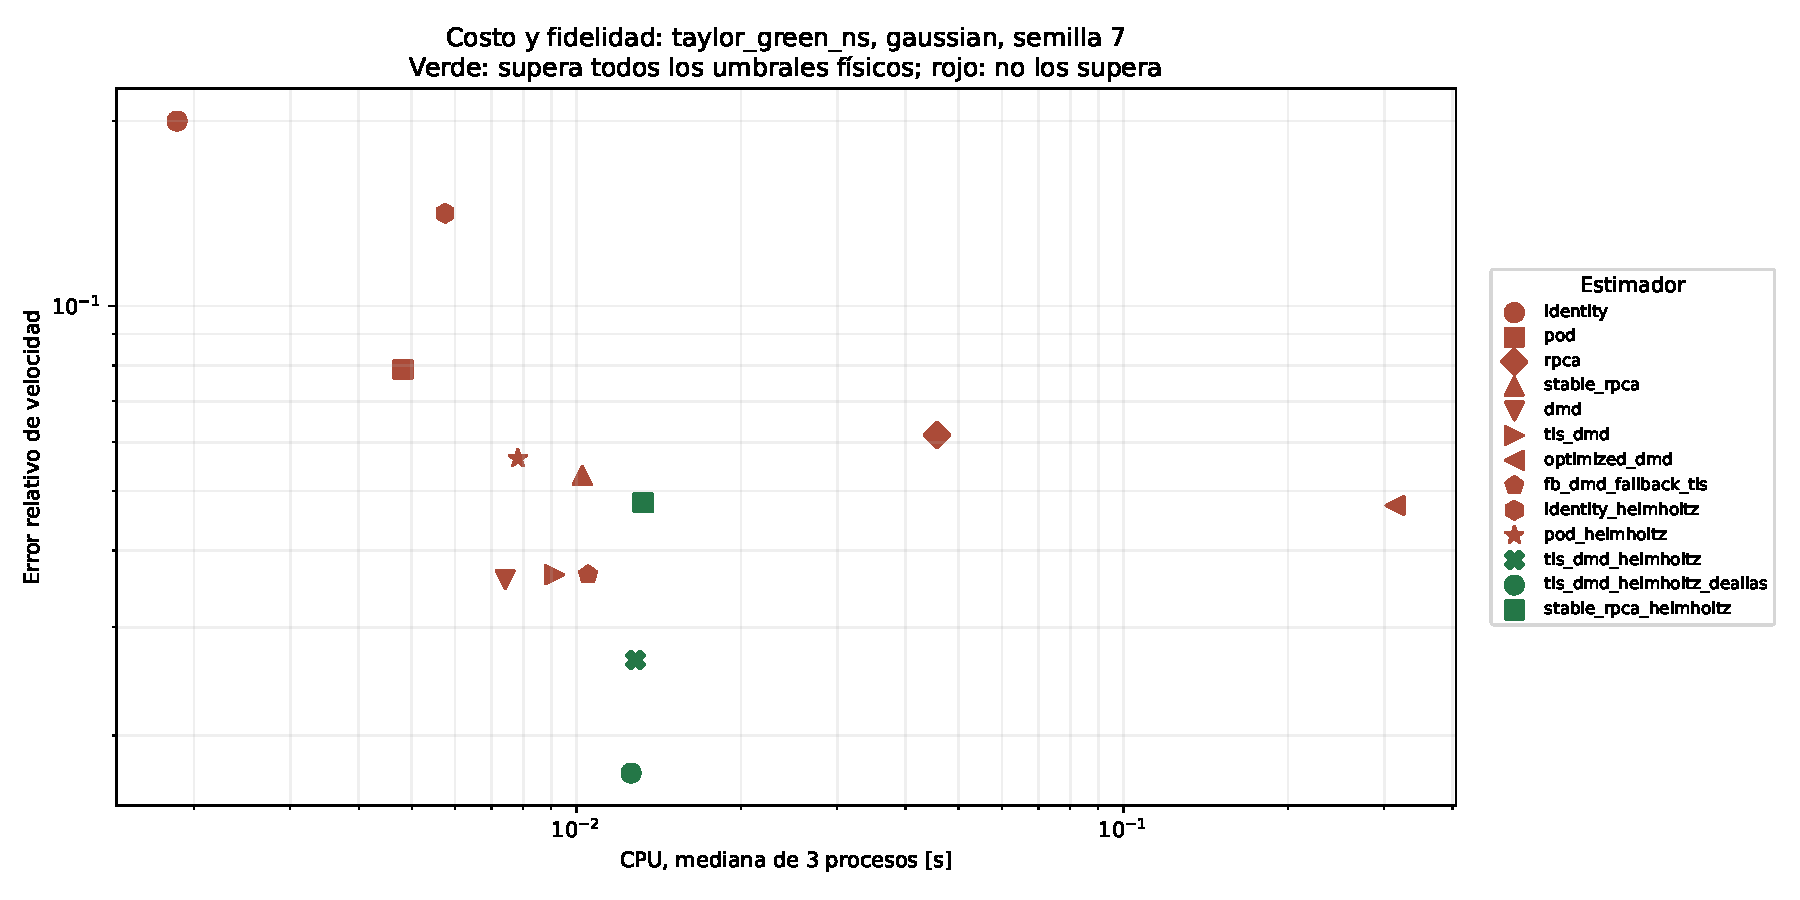
\includegraphics[width=.95\textwidth]{results/research/extended_physics_2026-10-14/figures/cost_quality.pdf}
\caption{Costo medido y error de velocidad en una condición coincidente. La aceptación incluye vorticidad, divergencia y energía; en canales, paredes.}\end{figure}
\section{Límites de la inferencia}
Las semillas son réplicas de contaminación del mismo campo; las repeticiones de recursos no aumentan el tamaño de muestra de calidad. La evaluación es reconstrucción dentro de la ventana, sin pronóstico ni mediciones PIV reales. El parámetro de ruido conocido es información del experimento sintético. Los perfiles HB estacionarios favorecen bajo rango temporal y no representan estelas; consulte los metadatos para distinguir perfiles de canales y solvers bidimensionales. La reconstrucción de velocidad no estima densidad: las métricas de masa y energía requieren densidad declarada. Los tiempos y métricas históricas de magnitud de velocidad no son directamente comparables a estas componentes vectoriales ni al entorno instrumentado.
Los CSV, ledger JSONL, configuraciones y hashes acompañan esta discusión en \texttt{results/research/extended\_\allowbreak physics\_\allowbreak 2026-10-14}. Las figuras de todos los casos se exportan a PNG y PDF; el resumen distingue convergencia y factibilidad física.
